\section{Introduction}

Programmers rely on online tutorials to pick up new skills and learn how to use frameworks and libraries.
This is an element of programmers' tendency to engage in interleaved programming and information foraging during programming tasks~\cite{brandt_two_2009}~\cite{brandt_example-centric_2010}.
However, online walkthroughs contain errors and incomplete information.
In the authors' experiences, they can lead to errors and fail to provide the conceptual knowledge the programmer will need to transfer online code to their own tasks.
\andrew{Not good enough.  How do we base this argument on more than our own intuitions?}
In the best case, this can cause a brief interruption in programming productivity.
In worse cases, it can cause frustration and confusion to the point of needlessly discouraging programming learners from learning new skills.
\andrew{Too general.  Concretify.}

Programmers increasingly use \emph{crowd documentation}~\cite{parnin_measuring_2011} found on the web that may be written by hobbyists without formal training writing usable documentation and who do not have QA resources to cross-check documents' quality.
\andrew{Can we back this up with concrete statistics?}
Tutorials provide an introduction to new concepts and hands-on practice with the tools that help programmers become comfortable performing new tasks.
\andrew{Give an example here.}
Unfortunately, even the best written tutorials have pitfalls.
They can't explain everything that the minimally-experienced user doesn't know, as they should maintain conciseness for more experienced readers and for a focus on the primary task at hand.
As programming tutorials assume a base understanding of at least one language or library, readers may come from a background that requires them to consult outside documentation.
A tutorial that walks one through a web scraping task may require an understanding of the Python language, callbacks, CSS selectors, regular expressions, and threading.
Gaining an understanding of any one of these prerequisites can be time-consuming.
It may even be difficult to grasp references to concepts like threads and processes if you don't know what they are when reading the tutorial.

\andrew{Before now, we should introduce the concrete examples from Figure~\ref{fig:tutorons}}

API method descriptions may be too abstract or vague to offer immediate understanding of unknown syntax or libraries.
Introductory documentation in a new domain may take too long to walk through to learn a supplemental skill to a primary task.

We build a \emph{new paradigm of programming documentation} between API descriptions and detailed, manually crafted walkthroughs.
\andrew{Where does this fall between?  Include a table with API method descriptions, tutorials, and tutorons, with trade-off dimensions including task relevance, adaptiveness to user background, level of detail, specificity to class, interactivity}.
In this paper, we propose \emph{\Glspl{name}, which are on-demand, context-relevant descriptions of programming grammars, commands and libraries} designed to be inserted within an existing tutorial to clarify the content of the tutorial, in a manner tailored to the reader's background knowledge and the particular task being accomplished in the tutorial.
\andrew{I'll have to think about how these can be tailored to the particular task being accomplished in the tutorial.}

\begin{figure}[!t]
\centering{
    \subfigure[Text augmentation explaining a CSS selector]{
        \framebox{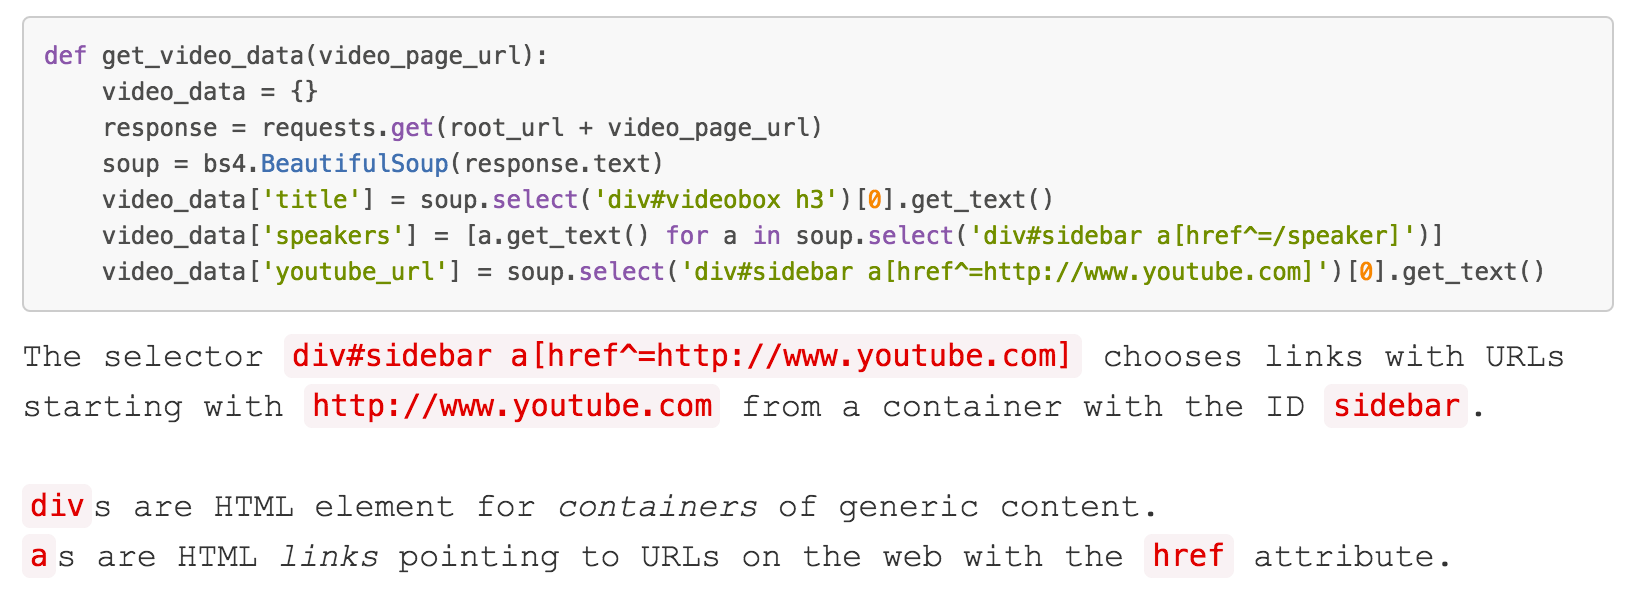
\includegraphics[width=.4\textwidth]{figures/css_explanation}}
        \label{fig:css_explanation}
    }
    \subfigure[Visualization and demonstration of regular expression]{
        \framebox{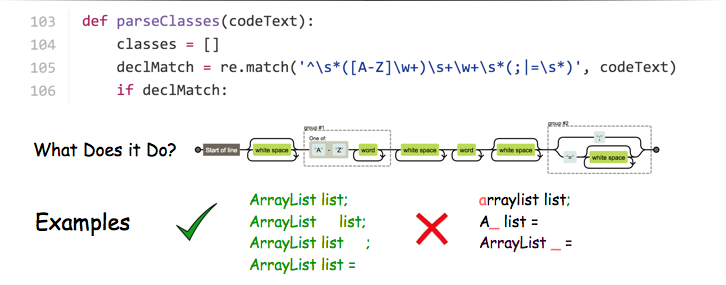
\includegraphics[width=.4\textwidth]{figures/regex_explanation}}
        \label{fig:regex_explanation}
    }
}
\label{fig:tutorons}
\caption{Automatic, context-relevant textual and visual explanations of code generated by descriptive \glspl{name}.}
\end{figure}

Automatic, context-relevant descriptions can take forms tailored to the code that needs to be explained, including simple text descriptions, code fragments and visualizations. 
We demonstrate how \glspl{name} of diverse types can produce just-in-time clarifications tailored to the domain and the communicative goal.
In particular, we consider \glspl{name} that can:
\begin{itemize} \itemsep1pt
\item generate text descriptions at multiple levels of detail
\item create domain-specific visualizations of code models
\item produce context-relevant usage examples
\item reinforce and clarify concepts from other \glspl{name}.
\end{itemize}

Implemtation steps include:
Pattern-matching heuristics for finding key examples of an explainable chunk of code.
Server-side code to generate explanations given a chunk of code.
Browser-based interactions for revealing adaptive explanations.
All of this can be done with Python and Java on a server, together with JavaScript on the front-end.
While we currently require custom JavaScript for each type of \gls{name} (natural language, visualization, etc.), in the future we could make templates of these types and reuse the same JavaScript for all \glspl{name}, requiring \glspl{name} authors to produce only server-side code to make explanations.

Ultimately, we believe \glspl{name} can speed up the process of interleaved web search for knowledge and code and implementation in the personal development environment~\cite{brandt} by reducing the number of resources programmers have to access to understand a tutorial.
\Glspl{name} can aid in such an ecosystem in three ways: tutorial reading, tutorial production, and code comprehension.
Through early user interface prototypes, we demonstrate how \glspl{name} will integrate into typical programming information seeking and coding practices.
We discuss the implications of this style of documentation for those writing programming documentation, highlighting the additional efforts needed and a sustainable framework for developing suites of context-relevant, on-demand comments.
To justify some of these expectations, we perform a preliminary evaluation to discover user perceptions of the helpfulness and relevance of \gls{name}-generated annotations.
We find that users who read \glspl{name}-produced explanations for regular expressions and wget commands results perform better on a multiple-choice activity asking them to report their understanding of these regular expressions and commands.

\subsection{Motivation}

Why do we need to help people seek information?
Programmers encounter problems reusing material online (Figure~\ref{fig:bad_tutorials}), that lead us to believe that tutorials should provide better support to:
\begin{itemize} \itemsep1pt
\item Help users recognize and overcome errors
\item Provide knowledge of best practices
\item Develop users' conceptual knowledge of their toolsets
\end{itemize}
Note that these are related to the tasks that Carroll describes in minimal instruction theory.

Recent studies reveal that programmers engage in opportunistic programming~\cite{brandt_two_2009}\cite{brandt_example-centric_2010}\cite{hartmann_hacking_2008}~\andrew{, which is...?}.
Both experienced programmers~\cite{duala-ekoko_asking_2012} and end-user programmers~\cite{dorn_lost_2013}\cite{dorn_learning_2010}\cite{rosson_everyday_2004} struggle to leverage web documentation to solve programming problems.
\andrew{TODO: read~\cite{dorn_learning_2010}\cite{rosson_everyday_2004}.}

Formally, we can look at these programming challenges as Ko et al.'s end-user programming learning barriers~\cite{ko_six_2004}.
For example, users may encounter the $selection$ barriers when trying to find APIs that will help them perform new tasks.
When troubleshooting the program, they may face the $understanding$ barrier to debug system output, or the $information$ barrier to try to learn more about silent failures.
Furthermore, programmers who develop a poor mental model of programming techniques~\cite{winslow_programming_1996} that they find online may find this to be an impediment during later learning.
\andrew{Make sure we're not misquoting the Winslow reference.}

\begin{figure*}[t]
\centering{
    \subfigure[The author of this tutorial assumes that readers of the tutorial are already literate in reading CSS selectors such as \texttt{div.foo li a}.]{
        \framebox{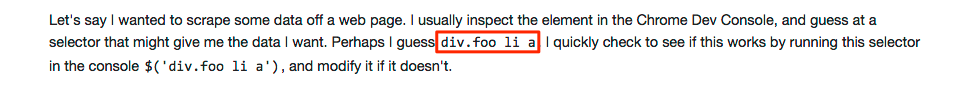
\includegraphics[width=.9\textwidth]{figures/css_bad}}
        \label{fig:css_bad}
    }
    \subfigure[The CascadeClassifer caused the paper's first author a great deal of grief in a past project due to the constructor's silent failure.  This caused him to experience an understanding barrier that could be avoided through a cv2-specific tutoron.]{
        \framebox{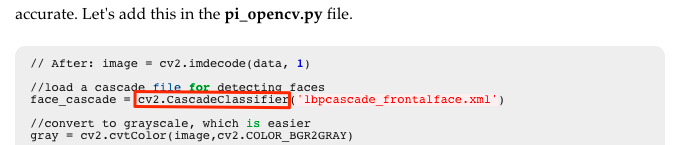
\includegraphics[width=.9\textwidth]{figures/cascadeclassifier_bad}}
        \label{fig:cascadeclassifier_bad}
    }
    \subfigure[A demonstration of scraping the web with \texttt{wget}.  Additional information on rate limiting could be helpful here to the eager tutorial learner who will instantly apply this technique.\bjoern{An interesting difference here is that you describe information that is NOT present in the command line. It strikes me as a harder problem to look for *absences* of code and determine whether this would be a good place to add it.}]{
        \framebox{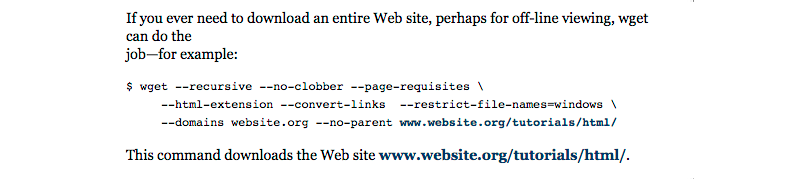
\includegraphics[width=.9\textwidth]{figures/wget_bad}}
        \label{fig:so_wget_bad}
    }
}
\caption{Three examples of online tutorials that can cause grief when followed.}
\label{fig:bad_tutorials}
\end{figure*}

\subsection{Background}

\subsubsection{How to Write Usable Technical Documentation}

We are inspired by minimal instruction theory, which provides guidelines for developing usable technical documentation~\cite{carroll_nurnberg_1990}.
There are three main insights of the minimalist approach:
learners are allowed to start immediatedly on meaningfully realistic tasks,
the amount of reading and other passive activity in training is reduced,
and errors and error recovery are presented in a way to make them less traumatic and more pedagogically productive.
Interstingly, today we find ourselves at a point where that much of the typical programming documentation is no longer developed by professionals.
Programmers increasingly use \emph{crowd documentation}~\cite{parnin_measuring_2011} found on the web that may be written by hobbyists without formal training writing usable documentation and who do not have QA resources to cross-check documents' quality.
\andrew{Is this the right reference for the term crowd documentation?}

When it is not possible to produce minimal instruction that has been iteratively tested and tailored to its audience, Farkas recommends \emph{layered documentation}~\cite{farkas_layering_1998}.
Layered documentation allows users to access more \emph{backup information} for tasks like error recognition and correction, and enables the same documentation to be used by readers from different backgrounds.
We position our work with the core belief that minimal instruction is a worthwhile but likely unattainable standard for online programming tutorials.
Given the diverse audiences of programming tutorials and the lack of documentation expertise of their authors, minimal instruction seems impossible to achieve.
We therefore adapt Farkas's advice with a technique for adding interactive layering to existing tutorial documentation on the web.
Through this, we approach the aims of minimal instruction: improved transfer of tutorial skills to personal tasks, less web search for discovering background knowledge, and faster error recovery.

Eiriksdottir \& Catrambone~\cite{eiriksdottir_procedural_2011} detail three types of instructions --- procedures, principles, and examples --- and their pedagogical aims.
Detailed procedures and relevant examples are likely to ease users' initial task performance.
More abstract procedures promote good learning and transfer.
We believe that \glspl{name} can improve relevance of more general procedures by providing just-in-time description of configurable parameters of APIs.
Furthermore, they can be used to describe relevant principles and interactive examples to aid transfer beyond the current task.

\subsubsection{What are the strengths and weaknesses of today's tutorials?}

Lafreniere et al.~\cite{lafreniere_understanding_2013} determined the type of activites that users engage in through comment-based discussion following the body of tutorials.
\andrew{What were the activities, how do people learn from tutorials, what are their weaknesses?}
In the programming domain, Parnin \& Treude~\cite{parnin_measuring_2011} find that 87.4\% of the methods of the jQuery API are described by a blog post in the first 10 web search results.
Of these blog posts, about half were tutorials.

In a survey of 154 Photoshop tutorials, Lount \& Bunt~\cite{lount_characterizing_2014} harvested tutorials from an application-centered community, tutorial aggregator, tutorial factory, and popular tutorials via the CUTS tecnique~\cite{fourney_characterizing_2011}.
Among other findings, Lount \& Bunt describe strengths and weaknesses of the corpus as a whole.
Almost all tutorials included source files (90.3\%), the initial image (91.6\%), final image (96.7\%), at least one image per step (84.4\%), and references to past steps when repeated steps were used (89.6\%).
However, 40.7\% of tutorials contained no attempts to address potential errors, 83.1\% omitted any version information, and only 1 of every 20 steps had any explanation.
Mechanisms to improve such tutorials' coverage of potential efforts and explanation of tools used could improve the quality of the average online tutorial.

\andrew{Also possibly relevant:~\cite{ames_just_2001}, for when and how to intervene with instructions.}


